\documentclass{article}
\usepackage{graphicx} % Required for inserting images
\usepackage[spanish]{babel}
\usepackage[colorlinks]{hyperref}
\usepackage{float}
\usepackage{multirow}
\usepackage{subfigure}

\title{TFG}
\author{JORDI PEREIRA GIL}
\date{Octubre 2024}

\begin{document}

\maketitle

\section{Introducción}
Aquí escribiendo la biblia

\begin{table}
    \centering
    \caption{Leyenda tabla}
\scriptsize
\begin{tabular}{|p{3cm}|p{3cm}|p{3cm}|p{3cm}|} \hline 
         \textbf{Característica}&  \textbf{Flutter}&  \textbf{Ionic}& \textbf{React navive}\\ \hline 
         Lenguaje de programación&  Dart&  JavaScript, HTML, CSS& JavaScript, TypeScript\\ \hline 
         Rendimiento&  Alto rendimiento (código nativo)&  Depende de WebView (más lento que nativo)& Cerca del rendimiento nativo\\ \hline 
         Acceso a APIs nativas&  Directamente mediante canales nativos&  Plugins nativos a través de Capacitor& Mediante módulos nativos o librerías\\ \hline 
         Facilidad de uso&  Curva de aprendizaje moderada (Dart)&  Fácil para desarrolladores web& Familiar para desarrolladores de JavaScript\\ \hline 
         Soporte multiplataforma&  iOS, Android, Web, Desktop&  iOS, Android, Web& iOS, Android\\ \hline 
         Componentes UI&  Propios y altamente personalizables&  Utiliza web components y plugins& Usa componentes nativos\\ \hline 
         Tamaño de la app&  Relativamente grande&  Más pequeño que Flutter& Relativamente pequeño\\ \hline 
         Licencia&  Open Source (BSD)&  Open Source (MIT)& Open Source (MIT)\\ \hline
    \end{tabular}
\caption{Comparativa tecnologías frontend}
\label{tab:my_table}
    
    
\end{table}


\chapter{Estado del Arte}

\section{Dominio del problema} \label{dompro}

En esta sección hablaremos más detalladamente del problema a resolver. 



Un actor clave en el sistema son las asociaciones de animales \cite{asociaciones}, éstas son entidades sin ánimo de lucro, legalmente constituidas cuyo fin principal es la protección y defensa de los animales, tanto de los animales de compañía como de los salvajes.

Técnicamente se conocen como «asociaciones de protección y defensa de los animales», aunque desde siempre las llamamos «protectoras de animales». Éstas se encargan, entre otras muchas tareas, de gestionar la adopción y acogida de los mismos. También suelen firmar convenios de colaboración con Comunidades autónomas y/o ayuntamientos para prestar servicios que estas administraciones no puedan prestar o no sean eficientes haciéndolos, como por ejemplo la recogida de animales callejeros.

Éstas se comunican mediante las redes sociales con las personas interesadas en realizar alguna de las acciones mencionadas previamente, esto lo sabemos gracias a la reuniones que tuvimos con Colonias Felinas de Armilla previas al desarrollo, las cuales además de proporcionarnos información para perfilar las tareas a realizar, también nos explicaron sobre su flujo de trabajo y como interactúan con la gente interesada. 

 Las asociaciones, generalmente no tienen demasiados ingresos, y deben utilizar herramientas de gestión gratuitas para ahorrar la mayor cantidad de dinero posible para utilizarlo con sus animales. Éstas no suelen ser muy completas como veremos en el apartado \ref{appssimilares}, haciendo necesario el uso de varias aplicaciones para la gestión de una sola entidad.

A coalición de esto, por ejemplo el proceso posterior a la adopción no suele ser controlado en este tipo de aplicaciones, haciendo que se tenga que recurrir a otras, como apps de mensajería u otras opciones para su gestión, lo cual produce un aumento la desorganización.

Como hemos mencionado anteriormente, la información acerca de los animales en adopción y/o acogida de una zona concreta está muy dispersa y se hace tediosa su búsqueda, esto sumado a lo indicado previamente, nos ha llevado a la conclusión que lo mejor sería centralizar dicha información en única aplicación.

Además, para los usuarios que decidan adoptar, es una buena idea que la aplicación les resulte familiar y manejable, en ese sentido creemos que el diseño debería ser similar al de las redes sociales actuales, ya que eso les resultaría atractivo y haría que, por lo menos una mayor cantidad de usuarios le diese una oportunidad a la aplicación. El objetivo de todo esto es que sea intuitiva teniendo que aprender lo menos posible para su uso, ya que si es muy complicada, éstos no querrán utilizarla.

Otra carencia en este ámbito, es la falta de gestión en los voluntariados. Esto suele ser algo común entre las asociaciones y protectoras, que no haya un registro de los voluntarios y su trabajo, y lo mismo ocurre con la propia gente que trabaja ahí, eso genera problemas de coordinación que serían fácilmente evitables si estuviesen registrados en alguna plataforma.

La idea es crear un sistema en que todas estas carencias sean suplidas en la medida de lo posible y ayudar tanto asociaciones y usuarios adoptantes, voluntarios y ciudadanos en general a tener una plataforma en la que poder compartir información sobre los animales.




\section{Revisión de tecnologías: alternativas} \label{rev}
En esta sección vamos a comparar las distintas tecnologías para el desarrollo de aplicaciones y entre todas las vistas podremos escoger las que sean más optimas para nuestro propósito. A continuación haremos una comparación entre los diferentes IDEs y tecnologías tanto para el cliente como para el servidor.

\subsection{IDEs}
Un entorno de desarrollo integrado (IDE) \cite{ide} es un sistema de software para el diseño de aplicaciones que combina herramientas del desarrollador comunes en una sola interfaz gráfica de usuario.

Como todavía no sabemos que lenguajes de programación vamos a utilizar, lo mejor es buscar entornos de desarrollo que acepten varios lenguajes, para ello nos decantaremos entre la suite de Jetbrains \cite{jetbrains} o Visual Studio Code \cite{vscode}:

\begin{table}[H]
	\centering

	\begin{tabular}{|>{\raggedright}p{3cm}|p{4cm}|p{4cm}|} 
		\hline
		\textbf{Característica} & \textbf{JetBrains (IntelliJ, PyCharm, etc.)} & \textbf{Visual Studio Code} \\ \hline
		Enfoque & IDE completo para lenguajes específicos & Editor de código ligero con extensibilidad \\ \hline
		Licencia & Comercial (gratis para estudiantes y OSS) & Código abierto \\ \hline
		Rendimiento & Más uso de recursos (IDE completo) & Ligero y rápido \\ \hline
		Integración & Herramientas integradas para cada lenguaje & Depende de extensiones \\ \hline
		Depuración & Depurador avanzado integrado & Depurador mediante extensiones \\ \hline
		Refactorización & Herramientas avanzadas de refactorización & Capacidades básicas de refactorización \\ \hline
		Precio & Pago (excepto versiones Community limitadas) & Gratuito \\ \hline
		Personalización & Limitada en comparación con VSCode & Altamente personalizable \\ \hline
		Extensiones & Ecosistema más limitado & Amplio mercado de extensiones \\ \hline
		Colaboración & Space (solución integrada) & Live Share (extensión) \\ \hline
		Inteligencia & AI Assistant (en versiones pagas) & Copilot (extensión de pago) \\ \hline
	\end{tabular}
		\caption{Comparación entre JetBrains Suite y Visual Studio Code}
\end{table}


\subsection{Cliente}

Primero hablaremos de las tecnologías para el cliente, para ello haremos uso de frameworks \cite{framework} que son estructuras conceptuales y tecnológicas de asistencia definida, normalmente, con artefactos o módulos concretos de software, que puede servir de base para la organización y desarrollo de software. Típicamente, puede incluir soporte de programas, bibliotecas, y un lenguaje interpretado, entre otras herramientas, para así ayudar a desarrollar y unir los diferentes componentes de un proyecto. A continuación se mostrán las siguientes alternativas: Flutter, Ionic y React Native.

\begin{table}[H] %Esto hace que se ponga donde le corresponde en lugar de "flotar"
    \centering
    \hspace*{-1.7cm}
    \begin{tabular}{|p{2cm} |p{4 cm} |p{4cm} |p{4cm} |} \hline 
         &  \textbf{Flutter}&  \textbf{Ionic}& \textbf{React Native}\\  \hline 
         Descripción &  Marco multiplataforma de código abierto de Google para desarrollar aplicaciones iOS/Android &  Marco frontend para crear aplicaciones móviles para teléfonos iOS/Android que utilizan la misma base de código& Framework de programación de aplicaciones nativas multiplataforma, para desarrollar apps iOS/Android\\ \hline 
         
        Lenguaje de programación &  Dart&  HTML,CSS y Javascript & Javascript\\ \hline 
        API nativas &  Sí&  Sí & Sí\\ \hline 
        Despliegue &  Móvil, Web, Escritorio&  Móvil, Web, PWA, Escritorio & Móvil\\ \hline 
        Rendimiento móvil &  Excelente &  Bueno & Muy bueno\\ \hline 
        Rendimiento web &  Deficiente &  Excelente & No tiene\\ \hline 
        Conocimiento previo & Bajo & Medio & Nulo \\ \hline
    \end{tabular}
    \caption{Comparativa tecnologías front-end \cite{flut-ion} \cite{flut-react}}
    \label{tab:tec_front}
\end{table}

\subsection{Servidor}

En cuanto al servidor, debemos separar entre las tecnologías de almacenamiento de datos y tecnologías de obtención y recepción de datos del cliente. A éstas últimas se les llama APIs \cite{api} son mecanismos que permiten a dos componentes de software comunicarse entre sí mediante un conjunto de definiciones y protocolos, en este caso al cliente con la base de datos. A continuación compararemos diferentes tipos de bases de datos y diferentes lenguajes para el servidor.

\subsubsection{Bases de datos}
Para la base de datos debemos saber que podemos elegir entre bases de datos relacionales (SQL) y no relacionales (NoSQL).

Las primeras están organizadas en tablas con filas y columnas. Usan un modelo relacional que funciona mejor con datos estructurados bien definidos, en los que existen relaciones entre las diferentes entidades.

En las NoSQL no se sigue un esquema rígido para el almacenamiento de los datos, éstas almacenan los datos en estructuras flexibles que suelen ser datos en formato JSON en unas entidades llamadas documentos, generalmente sin relación entre los mismos.\cite{sqlvsno}

A continuación vamos a comparar una de las bases de datos relacionales más populares con la base de datos no relacional más popular. 

\begin{table}[H] %Esto hace que se ponga donde le corresponde en lugar de "flotar"
    \centering
    \begin{tabular}{|p{2cm} |p{4 cm} |p{4cm} |} \hline 
         &  \textbf{MongoDb}&  \textbf{MySQL}\\  \hline 
         Tipo &  NoSQL &  SQL \\ \hline 
         
        Estructura de la base de datos &  Almacena los datos en documentos y colecciones de tipo JSON &  Almacena los datos en una estructura tabular con filas y columnas \\ \hline 
        Arquitectura &  Nexus &  Cliente servidor\\ \hline 
        Lenguaje de consulta &  MQL &  SQL\\ \hline
        Escalabilidad & Horizontal & Vertical \\ \hline
        Rendimiento & Alto rendimiento con grandes grupos de datos & Excelente para consultas y uniones de datos complejas \\ \hline 
        Seguridad &  Al no tener una estructura fija, pueden surgir incoherencias y problemas de seguridad de los datos &  ofrece una mayor seguridad ya que tiene estructuras de datos definidas con mayor consistencia \\ \hline
      	Integridad de los datos & No es muy consistente, es fácil que haya datos duplicados & Alta consistencia de datos \\ \hline
        Complejidad &  Fácil &  Muy fácil \\ \hline
        
    \end{tabular}
    \caption{Comparativa tecnologías BBDD \cite{sqlcomparison}}
    \label{tab:tec_db}
\end{table}


\subsubsection{Lenguajes de programación para el servidor}
En esta sección vamos a comparar los 3 principales lenguajes de programación de desarrollo para el servidor y sus frameworks más reconocidos: 
\begin{table}[H] %Esto hace que se ponga donde le corresponde en lugar de "flotar"
    \centering
    \begin{tabular}{|p{2cm} |p{3cm} |p{3cm} |p{3cm} |} \hline 
         &  \textbf{Javascript}&  \textbf{Python}& \textbf{PHP}\\  \hline 
         Framework &  Node.js &  Django & Laravel\\ \hline
         
        Conectividad BBDD &  Conectividad sencilla y con todo tipo de bases de datos&  La conectividad de la base de datos es posible, pero no para todos. Además, necesita controladores. & Conectividad sencilla, capaz de conectarse con más de 25 bases de datos sin problemas.\\ \hline 
        Curva de aprendizaje &  Muy fácil & Fácil & Media\\ \hline 
        Seguridad &  ofrece prácticas de seguridad que permiten securizar el sistema comodamente &  Más seguro con funciones de ciberseguridad integradas & Se han producido muchos ataques a la seguridad	\\ \hline 
        velocidad &  Más rápido que php &  Rápido(menos que php) & Muy rápido a partir de la versión 7\\ \hline 
        Popularidad & Un poco más popular que python 1.8\% &  Menos popular que PHP (alrededor del 1,1\% de todos los sitios de Internet utilizan Python) & Más popular (cerca del 79\% de los sitios web utilizan PHP)\\ \hline 
    \end{tabular}
    \caption{Comparativa tecnologías back-end }
    \label{tab:tec_back}
\end{table}

\section{Revisión de aplicaciones similares} \label{appssimilares}

En este apartado, vamos a revisar las tres aplicaciones más relevantes y usadas en el ámbito de la organización de las asociaciones y las adopciones. Estas son Amazdog, SukyCMS y Miwuki pet Center.

A continuación, vamos a describir las aplicaciones mencionadas anteriormente. Al final pondremos una tabla comparativa considerando las principales características que necesitamos que cubran según nuestros objetivos.

%ASPCA Volunteer Portal: https://play.google.com/store/apps/details?id=org.aspca.volunteer&pli=1
\begin{itemize}
	\item Amazdog \cite{amazdog}: Es una aplicación móvil en la cual se pueden adoptar animales y publicar si un animal se ha perdido. Además cuenta con servicios como búsqueda de playas que admiten mascotas y también proporcionan seguros para los animales.
	
\begin{figure}[H]
	\centering
	\includegraphics[width=0.7\linewidth]{"Sprint 0/amazdog"}
	\caption{Pantalla de inicio y de adopciones de la aplicación Amazdog}
	\label{fig:amazdog}
\end{figure}
	
	\item SukyCMS \cite{sukycms}: Es un gestor para las asociaciones de animales que cuenta con varios paneles de gestión en el que se destaca el del listado de animales que tiene en adopción la asociación. Esta aplicación, proporciona también la creación de una web a la que los usuarios pueden acceder para solicitar adopciones, además de ver información sobre la propia asociación.
	
	
\begin{figure} [H]
	\centering
	\includegraphics[width=0.7\linewidth]{"Sprint 0/sukycms"}
	\caption{Imagen de panel de administración de SukyCMS}
	\label{fig:sukycms}
\end{figure}
	
	\item Miwuki pet Center \cite{miwuki}: Este programa se encarga de la gestión de adopciones, acogidas y rescates de animales llevadas a cabo por protectoras, asociaciones, rescatistas y administraciones públicas. Una funcionalidad llamativa es la opción de realizar publicaciones automáticas en las principales redes sociales. 
	
	Por otra parte, el resto de usuarios pueden adoptar a los animales publicados por las distintas protectoras y filtrarlos por protectora específica. 
	 
\begin{figure}[H]
	\centering
	\includegraphics[width=0.7\linewidth]{"Sprint 0/miwuki"}
	\caption{Ejemplo de visualización de Miwuki}
	\label{fig:miwuki}
\end{figure}

\end{itemize}

\begin{table}[H] %Esto hace que se ponga donde le corresponde en lugar de "flotar"
	\centering
	\begin{tabular}{|p{5cm}|l|l|p{2.3cm}|} \hline 
		 & \textbf{Amazdog} & \textbf{SukyCMS} & \textbf{Miwuki} \\ \hline
		App móvil & Sí & No & Solo Android \\ \hline
		Versión web & No & Sí &  Sí \\ \hline
		Permite adopciones & Sí & Sí & Sí \\ \hline
		Permite acogidas & No & Sí & Sí \\ \hline
		Las asociaciones pueden pedir a particulares acoger a un animal & No & No & No \\ \hline
		Permite voluntariados & No & Sí & No \\ \hline
		Gestiona animales perdidos & Sí & No & No \\ \hline
		Gestiona animales encontrados & No & No & No \\ \hline
		Seguimiento post-adopción & No & No & No \\ \hline
		Ver el perfil de otros usuarios & No & No & Solo a protectoras \\ \hline
		Ver los animales de una protectora en especifico & No & No & Sí \\ \hline
		Buscar animales por zona & Sí & No & Sí \\ \hline
		Las asociaciones pueden recibir donaciones desde la app & No & No & No \\ \hline
		
		
		
    \end{tabular}
		\caption{Comparativa aplicaciones similares}
		\label{tab:appsSimilares}
	\end{table}
	
	Una vez revisadas y comparadas las distintas aplicaciones, podemos decir que la más completa es la de miwuki, cumpliendo con más requisitos que sus competidoras. No obstante, ninguna cubre con todas las funcionalidades deseadas, lo que refuerza la idea de crear una aplicación que aglutine todas estas características.
	
	Una funcionalidad interesante de miwuki, que añadiremos en nuestra aplicación, es la posibilidad de acceder al perfil de las protectoras y ver sus animales en adopción, además de una breve descripción de las mismas.  
\section{Propuesta}

\subsection{Descripción}

\subsection{Herramientas de desarrollo elegidas}

\subsection{Ciclo de vida/Metodología}
En esta sección hableremos de la métodología empleada, que en este caso hemos decidido usar la famosa metodología ágil scrum. \\

En este caso debido a la fluctuación temporal hemos decicido hacer sprints largos de un mes. Con esto tratamos de conseguir obtener un prototipo con cambios considerables a lo largo de cada sprint.


\subsection{Iteración 0}

Hablando con las asociaciones nos hemos dado cuenta de que los intercambios de acogidas no son una buena idea por lo que se ha descartado. \\
\subsubsection{Product Backlog}
Prioridades hechas con MoSCoW (tema 4 MDA)
\begin{table}[H]
    \centering
    \begin{tabular}{|c |p{8cm}|c |c|} \hline 
         \multirow[c]{3}{*}{Usuario}&  \textbf{Tarea}&  \textbf{Coste}& \textbf{Prio.}\\  \cline{2-4}%Prio. es de prioridad 
         &  Acceder a la aplicación&  5& M\\ \cline{2-4} 
         &  Cerrar sesión&  1& M\\ \hline 
    \end{tabular}
    \caption{Product backlog de usuarios}
    \label{tab:pb_usuarios}
\end{table}

\begin{table}[H]
    \centering
    \begin{tabular}{|c |p{8cm}|c |c|} \hline 
         \multirow[c]{23}{*}{Asociación}&  \textbf{Tarea}&  \textbf{Coste}& \textbf{Prio.}\\  \cline{2-4}
         
         &  Registrame en la aplicación como asociación&  5& M\\ \cline{2-4} 
         &  Poner animales en adopción&  8& M\\ \cline{2-4} 
         &  Anular poner animales en adopción&  3& M\\ \cline{2-4} 
         &  Ver solucitudes adopción&  5& M\\ \cline{2-4}
         &  Aceptar solucitudes adopción&  3& M\\ \cline{2-4}
         &  Rechazar solucitudes adopción&  3& M\\ \cline{2-4}
         
         
         &  Poner animales en acogida&  3& M\\ \cline{2-4}
         &  Anular poner animales en acogida&  3& M\\ \cline{2-4} 
         &  Ver solucitudes acogida&  3& M\\ \cline{2-4}
        
         &  Ver que usuarios tienen a sus animales en acogida&  5& M\\ \cline{2-4}
         &  Buscar usuarios que estén como casa de acogida&  5& M\\ \cline{2-4}
         &  Solicitar acogida a particular &  5& M\\ \cline{2-4}
         
         
         &  Decidir si desean ser voluntarios o no&  3& M\\ \cline{2-4}
         &  Ver solicitudes voluntariado propias&  3& M\\ \cline{2-4}
         &  Aceptar solucitudes voluntariado&  3& M\\ \cline{2-4}
         &  Rechazar solucitudes voluntariado&  3& M\\ \cline{2-4}
         
         &  Mandar contrato adopción firmado al adoptante&  8& S\\ \cline{2-4}
         
         &  Elegir si poner a sus animales como apadrinables o no &  5& S\\ \cline{2-4}
         &  Rechazar solucitudes voluntariado&  3& M\\ \cline{2-4}
         
         &  Modificar su descripción para que los usuarios vean a que se dedican & 5 & M \\ \hline

         
         
        
    \end{tabular}
    \caption{Product backlog de Asociaciones}
    \label{tab:pb_asociaciones}
\end{table}


\begin{table}[H]
    \centering
    \begin{tabular}{|c |p{8cm}|c |c|} \hline 
         \multirow[c]{14}{*}{Particular}&  \textbf{Tarea}&  \textbf{Coste}& \textbf{Prio.}\\  \cline{2-4}
         &  Registrame en la aplicación como particular&  5& M\\ \cline{2-4} 
         

         &  Solicitar adopciones&  3& M\\ \cline{2-4}
         &  Ver adopciones pendientes&  3& S\\ \cline{2-4}
         
         &  Solicitar acogidas&  3& M\\ \cline{2-4} 
         &  Ver acogidas pendientes&  3& M\\ \cline{2-4}
       
         &  Ponerse como casa de acogida&  3& S\\ \cline{2-4}
         
         &  Cumplimentar el formulario de solicitud de adopciones/acogidas &  5& S\\ \cline{2-4}
		 &  Firmar contrato de adopción electrónicamente&  8& S\\ \cline{2-4}
		 
		 
         &  Solicitar voluntariados&  3& M\\ \cline{2-4} 
         &  Ver voluntariados pendientes&  3& M\\ \cline{2-4}
         &  Ver historial voluntariados&  5& C\\ \cline{2-4}
         
         
         & Apadrinar a un animal&  5& S\\ \hline
         
         
         
    \end{tabular}
    \caption{Product backlog de Particulares}
    \label{tab:pb_particulares}
\end{table}

\begin{table}[H]
    \centering
    \begin{tabular}{|c |p{8cm}|c |c|} \hline 
         \multirow[c]{17}{2cm}{Asociación y Particular}&  \textbf{Tarea}&  \textbf{Coste}& \textbf{Prio.}\\  \cline{2-4}

         &  Ver su perfil &  5& M\\ \cline{2-4}
         &  Modificar su perfil &  5& M\\ \cline{2-4}
         &  Eliminar su perfil &  3& M\\ \cline{2-4}
         
         &  Aceptar solucitudes acogida&  3& M\\ \cline{2-4}
         &  Rechazar solucitudes acogida&  3& M\\ \cline{2-4}
         
         &  Ver historial de adopciones &  5& M\\ \cline{2-4}
         &  Ver historial de acogidas &  5& M\\ \cline{2-4}
         &  Eliminar sus publicaciones &  3& M\\ \cline{2-4}
         
         & Poner aviso de animal perdido encontrado & 5 & M \\ \cline{2-4}
         & Ver lista de animales perdidos & 5 & M \\ \cline{2-4}

         &  Reportar un perfil &  1& M\\ \cline{2-4}
         &  Reportar una publicación &  1& M\\ \cline{2-4}
         
         &  Realizar el seguimiento de adoción de la mascota adoptada&  8& C\\ \cline{2-4}
         
         &  Chatear con otros usuarios a raiz de una adopción/acogida/voluntariado &  8& M\\ \hline

         
         
    \end{tabular}
    \caption{Product backlog de Particulares y Asociaciones}
    \label{tab:pb_aso_particular}
\end{table}

\begin{table}[H]
    \centering
    \begin{tabular}{|c |p{8cm}|c |c|} \hline 
         \multirow[c]{4}{2cm}{Us. Básico y Particular}&  \textbf{Tarea}&  \textbf{Coste}& \textbf{Prio.}\\  \cline{2-4}
         
		 &  Buscar anuncios en una zona concreta&  5& S\\ \cline{2-4}		
         &  Ver peticiones de adopción&  8& M\\ \hline

         
         
    \end{tabular}
    \caption{Product backlog de Us. Básico y Particulares}
    \label{tab:pb_part_usBasico}
\end{table}

\begin{table}[H]
    \centering
    \begin{tabular}{|c|p{8cm}|c|c|} \hline 
         \multirow[c]{4}{*}{Administrador}&  \textbf{Tarea}&  \textbf{Coste}& \textbf{Prio.}\\  \cline{2-4}
         &  Crear usuarios &  5& M\\ \cline{2-4}
         &  Modificar usuarios &  5& M\\ \cline{2-4}
         &  Eliminar usuarios &  3& M\\ \hline

         
         
    \end{tabular}
    \caption{Product backlog de Administradores}
    \label{tab:pb_administradores}
\end{table}

\begin{table}[H]
    \centering
    \begin{tabular}{|c|p{8cm}|c|c|} \hline 
         \multirow[c]{7}{*}{Moderador}&  \textbf{Tarea}&  \textbf{Coste}& \textbf{Prio.}\\  \cline{2-4}
         &  Ver publicaciones reportadas &  5& M\\ \cline{2-4}
         &  Eliminar publicaciones reportadas &  3& M\\ \cline{2-4}

         &  Ver usuarios reportados &  5& M\\ \cline{2-4}
         &  Banear usuarios reportados &  3& M\\ \cline{2-4}
         
         &  Ver lista de asociaciones recién registradas &  5& M\\ \cline{2-4}
         &  Validar las asociaciones recién registradas& 5 & M\\ \hline

         
         
    \end{tabular}
    \caption{Product backlog de Moderadores}
    \label{tab:pb_moderadores}
\end{table}

Una vez creadas todas las historias de usuario procedemos a su planificación y asignación en los diferentes sprints, la idea es hacer un scrum con sprints de un mes. A continucación se muestran las tareas asignadas a cada sprint: \\ \\

Sprint 1 \\ 
\begin{figure}[H]
	\centering
	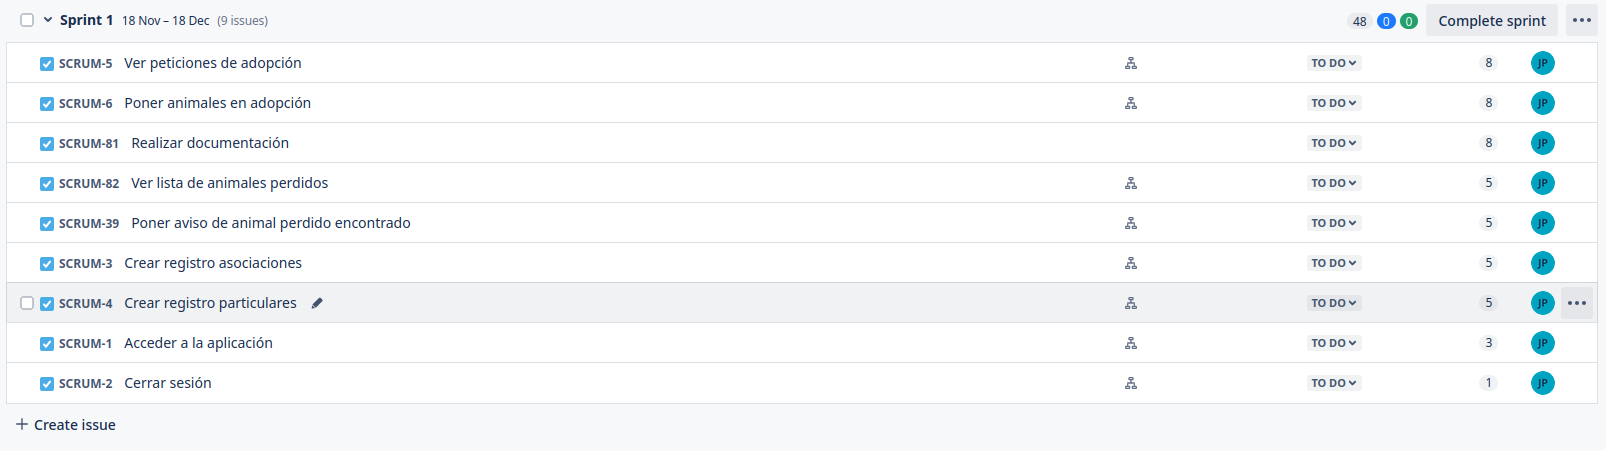
\includegraphics[width=1\linewidth]{screenshot001}
	\caption{Planificación del primer sprint}
	\label{fig:sprint1}
\end{figure}


Sprint 2 \\
\begin{figure}[H]
	\centering
	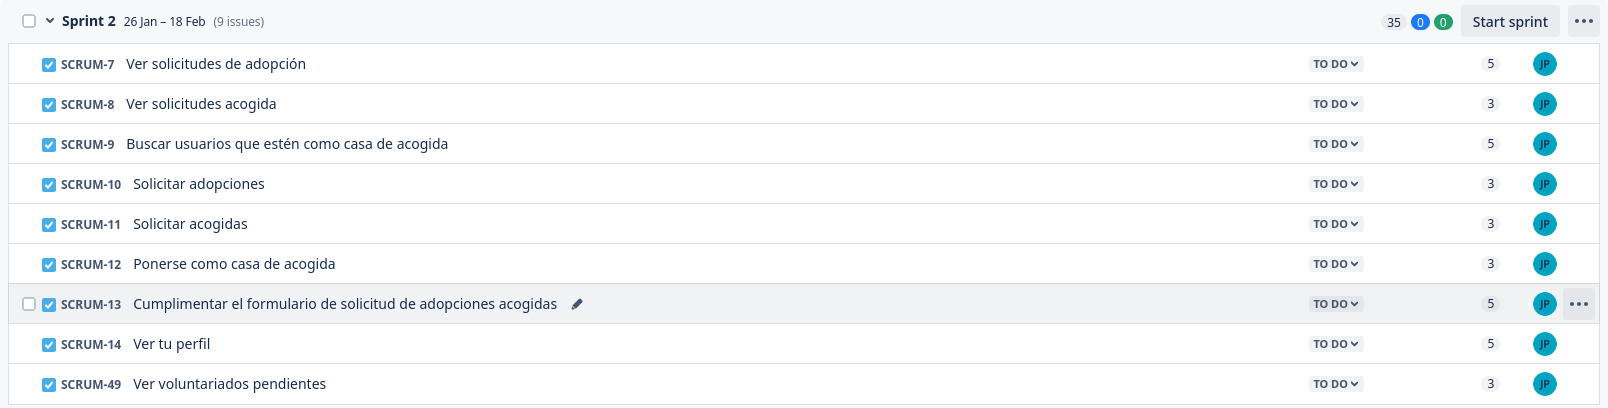
\includegraphics[width=1\linewidth]{screenshot002}
	\caption{Planificación del segundo sprint}
	\label{fig:sprint2}
\end{figure} 


Sprint 3 \\ 
\begin{figure}[H]
	\centering
	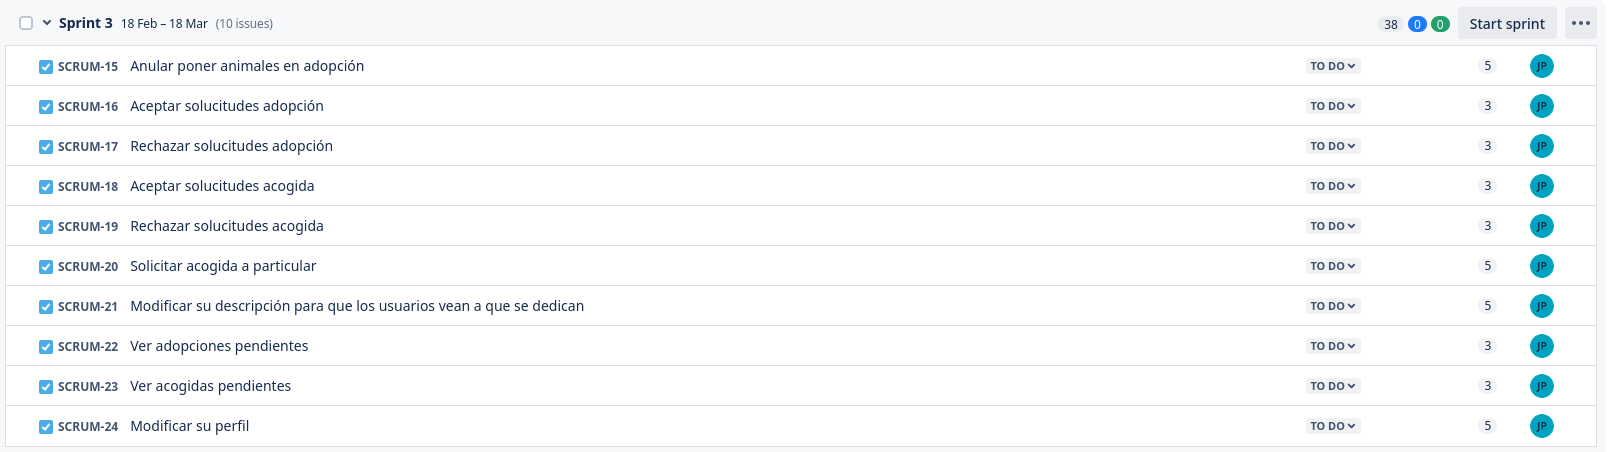
\includegraphics[width=1\linewidth]{sprint3}
	\caption{Planificación del tercer sprint}
	\label{fig:sprint3}
\end{figure}

Sprint 4 \\
\begin{figure}[H]
	\centering
	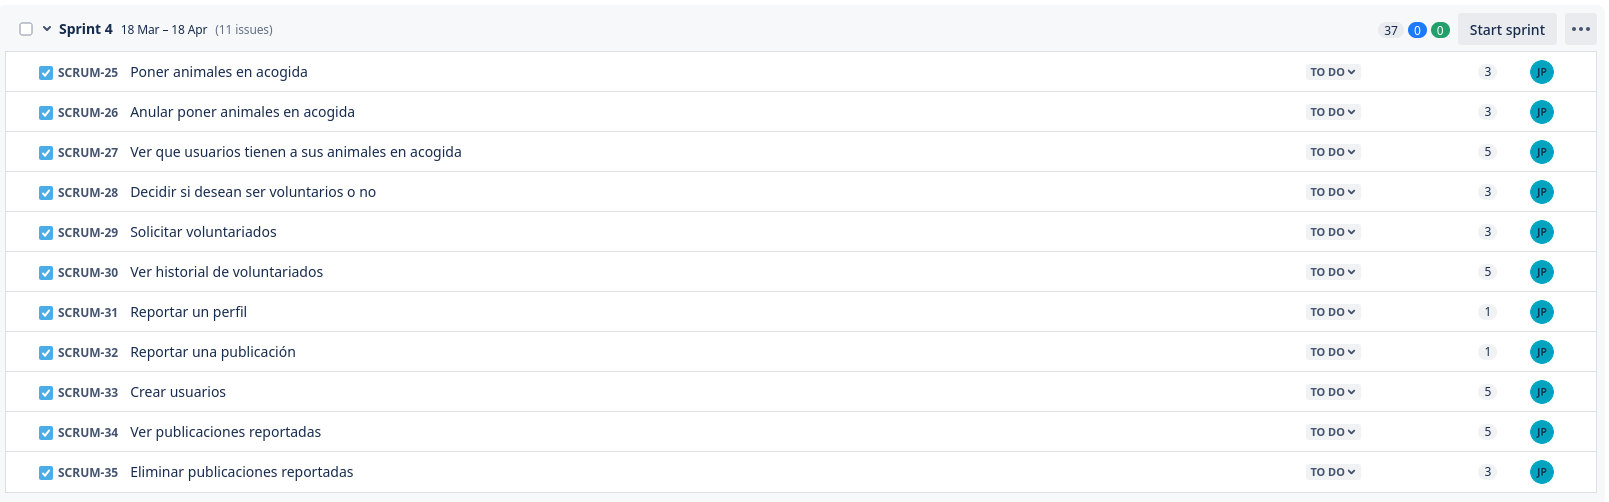
\includegraphics[width=1\linewidth]{sprint4}
	\caption{Planificación del cuarto sprint}
	\label{fig:sprint4}
\end{figure}

Sprint 5 \\ 
\begin{figure}[H]
	\centering
	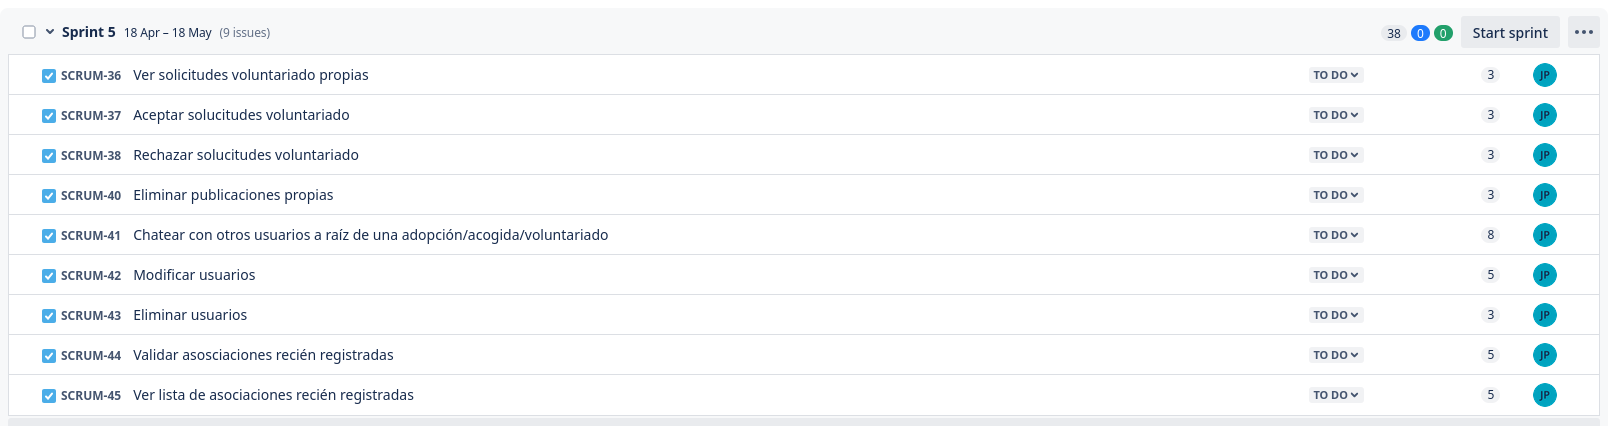
\includegraphics[width=1\linewidth]{sprint5}
	\caption{Planificación del quinto sprint}
	\label{fig:sprint5}
\end{figure}

Porduct backlog restante \\
\begin{figure}[H]
	\centering
	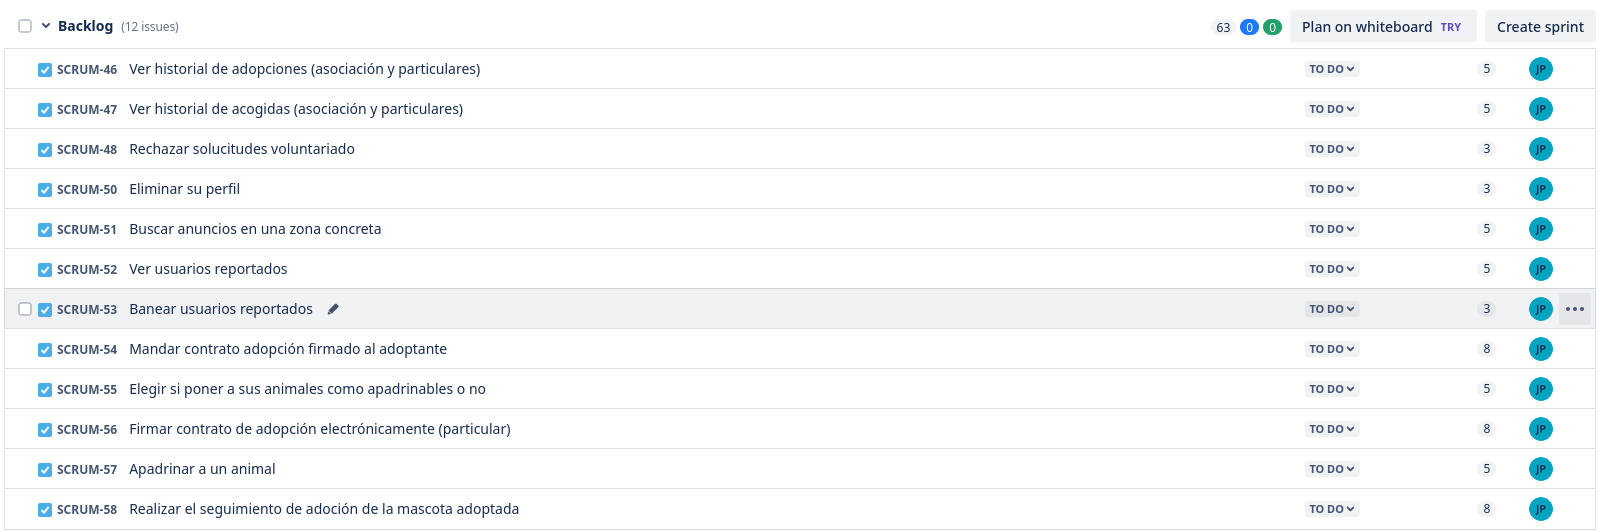
\includegraphics[width=1\linewidth]{pb}
	\caption{Tareas a hacer en siguientes sprints}
	\label{fig:pb_restante}
\end{figure}





\subsection{Iteración 1}

\large{\textbf{Especificación de tareas}} \\


\begin{tabular}{|c|p{9.5cm}|p{1cm}|}
	\hline
	\multicolumn{3}{|c|}{\textbf{HU.1 - Ver animales en adopción}} \\
	\hline
	\textbf{Id} & \textbf{Título de la tarea de desarrollo} & \textbf{Est. (días)} \\
	\hline
	1.1 & Realizar bocetos & 0.5 \\ \hline
	1.2 &  Implementar interfaz para ver las adopciones disponible & 2 \\ \hline
	1.3 &  Implementar la lógica de obtención de animales en adopción & 1 \\ \hline
	\multicolumn{3}{|c|}{\textbf{Pruebas de aceptación}} \\ \hline
	1 & \multicolumn{2}{|l|}{Mostrar mensaje en caso de que no haya animales} \\ \hline
	2 & \multicolumn{2}{|l|}{Mostrar lista de todos los animales} \\ \hline
	3 & \multicolumn{2}{|l|}{Que los filtros funcionen correctamente} \\ \hline
	
\end{tabular} \\ \\

\label{sec:hu1}

\begin{tabular}{|c|p{9.5cm}|p{1cm}|}
	\hline
	\multicolumn{3}{|c|}{\textbf{HU.2 - Poner animales en adopción}} \\
	\hline
	\textbf{Id} & \textbf{Título de la tarea de desarrollo} & \textbf{Est. (días)} \\ %Est. es estimación
	\hline
	2.1 & Realizar bocetos & 0.5 \\ \hline
	2.2 &  Implementar interfaz para añadir animales en adopción & 2 \\ \hline
	2.3 &  Insertar datos de animales en la bd & 2 \\ \hline 
	\multicolumn{3}{|c|}{\textbf{Pruebas de aceptación}} \\ \hline
	1 & \multicolumn{2}{|l|}{Mostrar avisos en caso de error en el fomulario} \\ \hline
	2 & \multicolumn{2}{|l|}{Previsualizar imágenes asociadas al animal} \\ \hline
	3 & \multicolumn{2}{|l|}{Poder eliminar imágenes concretas antes subirlas al servidor} \\ \hline
\end{tabular} \\ \\


\begin{tabular}{|c|p{9.5cm}|p{1cm}|}
	\hline
	\multicolumn{3}{|c|}{\textbf{HUT.1 - Realizar documentación}} \\
	\hline
	\textbf{Id} & \textbf{Título de la tarea de desarrollo} & \textbf{Est. (días)} \\
	\hline
	1.1 & Realizar documentación para cada tarea & 3 \\ \hline
	1.2 &  Añadir tareas a las historias de usuario & 0.5 \\ \hline
\end{tabular} \\ \\

\begin{tabular}{|c|p{9.5cm}|p{1cm}|}
	\hline
	\multicolumn{3}{|c|}{\textbf{HUT.2 - Aprender las tecnologías a utilizar}} \\
	\hline
	\textbf{Id} & \textbf{Título de la tarea de desarrollo} & \textbf{Est. (días)} \\
	\hline
	2.1 & Buscar documentación sobre sequelize & 1.5 \\ \hline
	2.2 & Buscar documentación sobre Ionic & 1.5 \\ \hline
\end{tabular} \\ \\


Una vez planificadas todas las historias de usuario del sprint empezaremos a realizarlas preferentemente en el orden designado. \\ \\

\Large{\textbf{HU.1 - Ver animales en adopción}} \\

En esta historia nos encargamos de la visualización de los distintos animales de adopción y su filtrado en función a unos parámetros clave, en este caso se han elegido la edad, la especie, y la localización. \\

Además por otra parte cabe destacar que esta será la página principal para los usuarios particulares. \\ 

\textbf{Bocetos}

Lo primero es crear los bocetos de la página para ello hemos hecho uso de la herramienta draw.io la cual permite realizar bocetos simples en poco tiempo.

\begin{figure}[H]
	\centering
	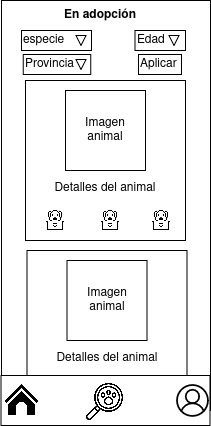
\includegraphics[width=0.31\linewidth]{"bocetos/iteracion 1/adopciones.drawio"}
	\caption{Boceto de visualización de animales en adopción}
	\label{fig:adopciones}
\end{figure}

Como podemos ver la idea para la página es mostrar una lista con los animales en busqueda de adopción en un contenedor con el siguiente formato:

\begin{itemize}
	\item \textbf{Imágenes de los animales}: Esto será un carrousel de imágenes en el que las asocaciones podrán mostrar el aspecto físico de sus animales.
	\item \textbf{Información específica}: Aquí se encontarán datos como el nombre, la raza y la edad del animal además de una descripción sobre el mismo.
	\item \textbf{Botones de acción}: las diferentes acciones a realizar serían la de solicituda de adopción, solicitud de acogida y apadrinamiento. Solicitud y apadrinamiento aparecerán solo si quiere la asocicación y este último tampoco aparecerá si ya está apadrinado.
\end{itemize}

\textbf{Implementación} %dimensiones móvil 506x901 \\

\begin{figure}[H]
		\centering
		\includegraphics[width=0.5\linewidth]{"Diseños finales/Iteracion 1/adopciones"}
		\caption{Vista final de la página que muestra a los animales en adopción en móviles}
		\label{fig:adopcionesDef}
\end{figure}


\begin{figure}[H]
	\centering
	\includegraphics[width=0.8\linewidth]{"Diseños finales/Iteracion 1/adopciones_web"}
	\caption{Vista final de la página que muestra a los animales en adopción en web}
	\label{fig:adopcionesDefWeb}
\end{figure}

Como podemos apreciar en ambos diseños se mantienen los componentes principales que mencionamos en los bocetos. Se ha usado el elemento de \textit{ion-card} para cada animal y en el se han añadido las imágenes pertinentes y una descripción del mismo.

A diferecia de la versión móvil, en web para que el espacio no esté totalmente vacío se ha decidido poner 2 tarjetas por fila, manteniendo su legibilidad y organización básica. \\


\textbf{Detalles de Implementación}

En esta sección comentaremos los elementos más importantes del desarrollo para el correcto funcionamiento de la HU, podremos hablar de funciones específicas en el código o de decisiones tomadas durante su realización. \\

Para esta HU hemos tenido que crear las tablas en la base de datos de animales, usuarios de tipo asociación, pasíses y provincias, este último para poder hacer funcionar el filtro de localizaión para la búsqueda de adopciones. \\

En cuanto al servidor se han tenido que crear funciones para obtener a todos los animales o buscarlos en función de los filtros utilizados. \\

En la parte del cliente básicamente se ha creado la pantalla de vista de animales y un servicio el cual nos permite conectarnos al servidor para hacer las peticiones de obtención tanto de filtros como de las adopciones. \\ 



\Large{\textbf{HU.2 - Poner animales en adopción}}

En esta historia nos encargamos de de la subida de animales en adopción a la plataforma para que los distintos usuarios los puedan visualizar. \\

\textbf{Bocetos}

\begin{figure}[H]
	\centering
	\includegraphics[width=0.31\linewidth]{"bocetos/iteracion 1/poner-adopción.drawio"}
	\caption{Boceto de página para añadir animales en adopción}
	\label{fig:poner-adopcion}
\end{figure}

Podemos apreciar que en esta página será básicamente un formulario que se divide en 3 partes diferenciadas: \\ 

\begin{itemize}
	\item \textbf{Datos básicos}: Este apartado contendrá la información necesaria (nombre, edad, especie, etc.) del animal en cuestión.
	\item \textbf{Imágenes}: En este apartado se pondrán las fotos que se quiera.
	\item \textbf{Datos específicos}: Estos son un conjunto de \textit{checkboxes} en los que se dará informción mas detallada y clínica sobre tratamientos a los que haya sido sometidos como por ejemplo castración o desparasitación entre otros.
\end{itemize}

\textbf{Implementación} \\

\begin{figure}[H]
	\centering
	\includegraphics[width=0.7\linewidth]{"Diseños finales/Iteracion 1/subidaAdopciones"}
	\caption{ Diseño de subida de adopciones móvil}
	\label{fig:subidaadopciones}
\end{figure}


\begin{figure}[H]
	\centering
	\includegraphics[width=0.7\linewidth]{"Diseños finales/Iteracion 1/subAdopWeb"}
	\caption{Diseño de subida de adopciones web}
	\label{fig:subadopweb}
\end{figure}

Como podemos apreciar en diferencia con el boceto los campos básicos aparecen en vértical de uno en uno en lugar de ir por bloques, esto se ha decido para aportar mayor legibilidad y orden, ya que de la otra manera tendrían tamaños irregulares y en ciertos modelos de teléfono probablemnete hubiese errores de superposción de elementos. \\


\textbf{Detalles de implementación} \\

Para esta historia de usuario se ha modificado la tabla de animales para añadir los campos del checkbox y su correspondiente actualización en el backend. También hemos creado sendos métodos para la subida de imágenes, que se guardan en la carpeta uploads del servidor y se enlaza con una tupla en la tabla \textit{images} en la base de datos la cual contiene su nombre, y animales. En caso de que no se puedan añadir las imágenes se borrará de la base de datos al animal y se le avisará al usuario de que ha habido un error. \\


En cuanto al frontend hemos creado una página nueva en el proyecto la cual contiene un formulario y hemos hecho uso de FormGrup de Angular el cual nos permite hacer validaciones básicas como por ejemplo que una cadena tenga x caracteres, también se ha creado una función de validación de campos en la que se le da información al usuario de los errores mediante un elemento \textit{Toast}. \\

Por último se han creado también funciones para la obtención de imágenes que puede ser tanto desde la galería como desde la cámara en su versión móvil y solo desde los archivos en la versión web y la posibilidad de eliminar imágenes en caso de que no las queramos antes de la subida de los animales.\\

\textbf{Fin del Sprint}

\begin{enumerate}
	\item Velocidad del Sprint \\ \\
	Como bien se puede ver en la tabla del sprint 0 se habían planificado una serie de tareas para este mismo, pero una vez terminado debemos hacer una reestimación de la velocidad ya que el aprendizaje e investigación de las tecnologías ha suspuesto más tiempo del esperado, produciendo así retrasos en la realización de las tareas. Debido a esto la planificación estimada de los siguientes sprints quedaría de la siguiente manera: \\
	
	Sprint 2 \\
	\begin{figure}[H]
		\centering
		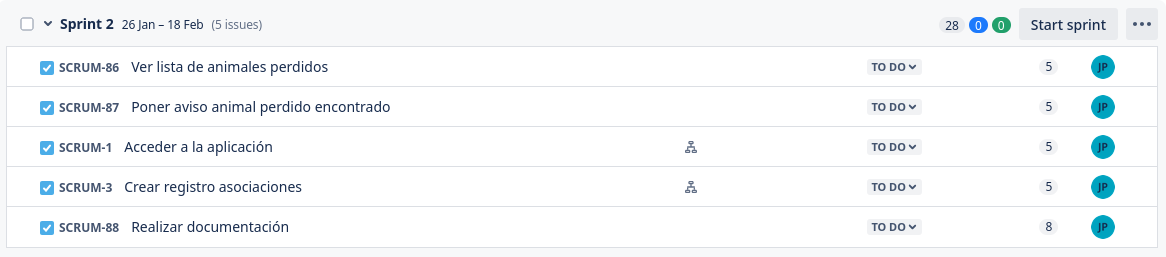
\includegraphics[width=1\linewidth]{newSprint2}
		\caption{Nuevas tareas sprint 2}
		\label{fig:newsprint2}
	\end{figure}
	
	
	Sprint 3 \\
	\begin{figure}[H]
		\centering
		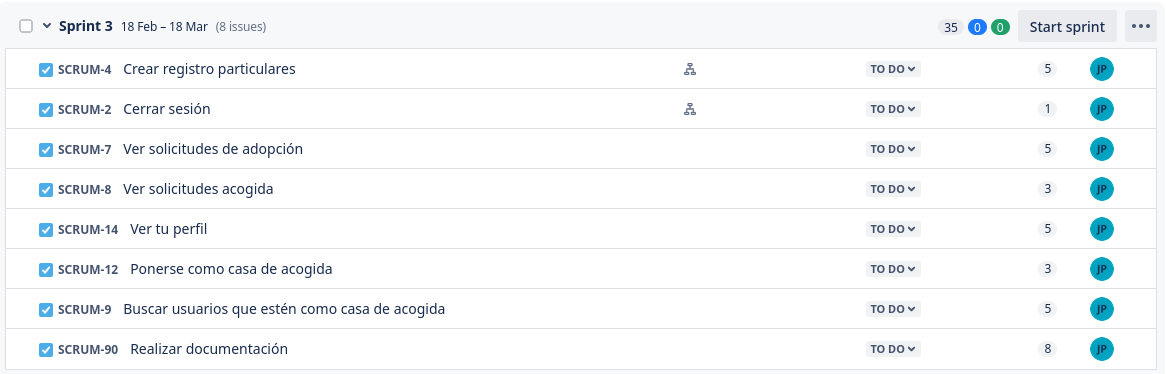
\includegraphics[width=1\linewidth]{newSprint3}
		\caption{Nuevas tareas sprint 3}
		\label{fig:newsprint3}
	\end{figure}
	
	Sprint 4 \\
	\begin{figure}[H]
		\centering
		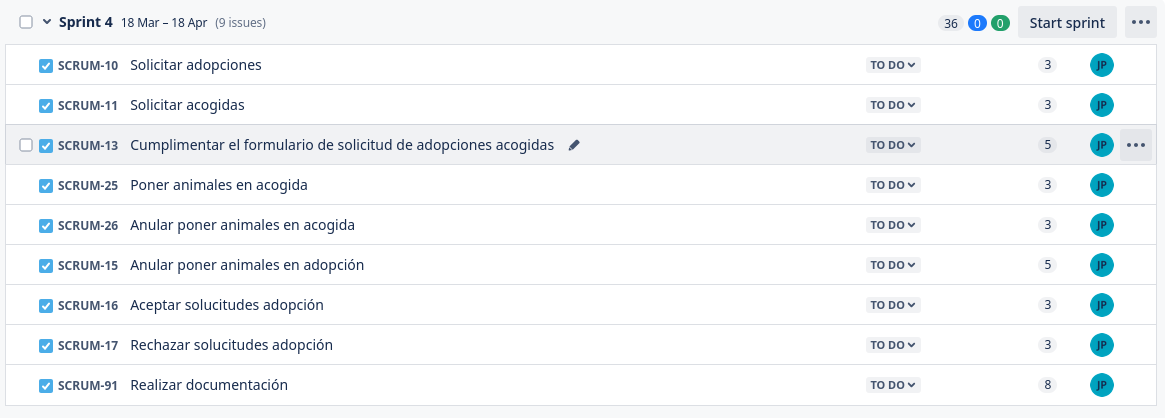
\includegraphics[width=1\linewidth]{newSprint4}
		\caption{Nuevas tareas sprint 4}
		\label{fig:newsprint4}
	\end{figure}
	
	
	Sprint 5 \\ 
	\begin{figure}[H]
		\centering
		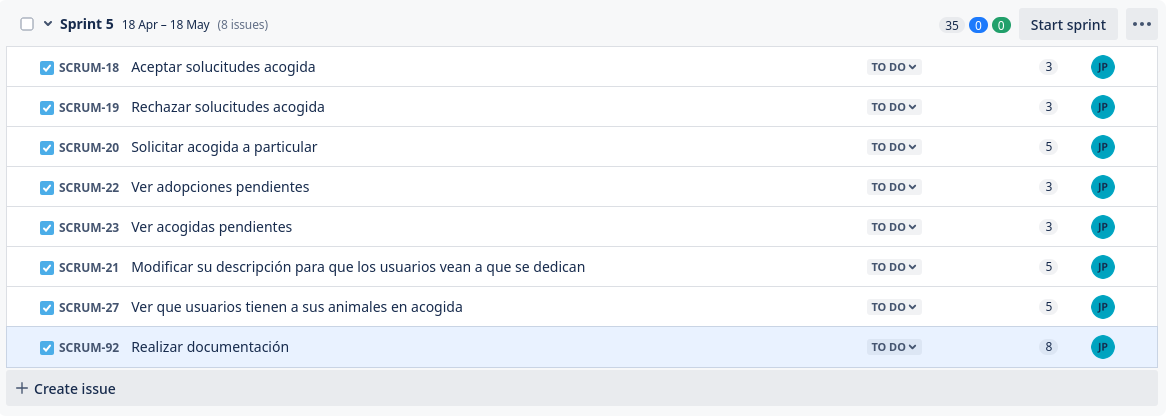
\includegraphics[width=1\linewidth]{newSprint5}
		\caption{Nuevas tareas sprint 5}
		\label{fig:newsprint5}
	\end{figure}
	
	El resto de tareas se moverán al backlog para su futura realización.
	
	\item Backend
	
	Como hemos visto en apartados anteriores (explicar en descripción de la propuesta que uso modelo-vista-controlador) en el back se encuentran tanto los controladores como los modelos para el acceso a la base de datos y su envío a la aplicación móvil. \\
	
	En la finalización del primer sprint la estructura de directorios es la siguiente:
	
	\begin{figure}[H]
		\centering
		\includegraphics[width=0.7\linewidth]{"sprint 1/directoriosBack"}
		\caption{Estructura de directorios del backen al final del sprint}
		\label{fig:directoriosback1}
	\end{figure}
	
	Además al utilizar un ORM se accede a la base de datos mediante clases por lo que para ilustrar su estructura se ha realizado un diagrama con sus relaciones y funciones básicas:
	
	\begin{figure}[H]
		\centering
		\includegraphics[width=1\linewidth]{"sprint 1/clases"}
		\caption{Diagrama de clases de la primera iteración}
		\label{fig:clases}
	\end{figure}
	
\end{enumerate}


\subsection{Iteración 2}
\large{\textbf{Especificación de tareas}} \\

\begin{tabular}{|c|p{9.5cm}|p{1cm}|}
	\hline
	\multicolumn{3}{|c|}{\textbf{HU.3 - Ver lista de animales perdidos}} \\
	\hline
	\textbf{Id} & \textbf{Título de la tarea de desarrollo} & \textbf{Est. (días)} \\
	\hline
	3.1 & Realizar bocetos & 0.5 \\ \hline
	3.2 &  Implentar la lógica de acceso a los animales perdidos & 2 \\ \hline
	3.3 &  Implementar la interfaz para subir el aviso & 1 \\ \hline
	\multicolumn{3}{|c|}{\textbf{Pruebas de aceptación}} \\ \hline
	1 & \multicolumn{2}{|l|}{Mostrar mensaje en caso de que no haya animales perdidos} \\ \hline
	2 & \multicolumn{2}{|l|}{Mostrar lista de todos los animales perdidos} \\ \hline
	3 & \multicolumn{2}{|l|}{Que los filtros funcionen correctamente} \\ \hline
\end{tabular} \\ \\


\begin{tabular}{|c|p{9.5cm}|p{1cm}|}
	\hline
	\multicolumn{3}{|c|}{\textbf{HU.4 - Poner aviso de animal perdido encontrado}} \\
	\hline
	\textbf{Id} & \textbf{Título de la tarea de desarrollo} & \textbf{Est. (días)} \\
	\hline
	4.1 & Realizar bocetos & 0.5 \\ \hline
	4.2 &  Actualizar la logíca para añadir avisos a la base de datos & 2 \\ \hline
	4.3 &  Implementar la interfaz para subir el aviso & 1 \\ \hline
	\multicolumn{3}{|c|}{\textbf{Pruebas de aceptación}} \\ \hline
	1 & \multicolumn{2}{|p{10cm}|}{Comprobar que los campos deben estar cumplimentados antes de realizar la petición} \\ \hline
	2 & \multicolumn{2}{|p{10cm}|}{Que la imagen recortada se almacena apropiadamente} \\ \hline
	3 & \multicolumn{2}{|p{10cm}|}{Que la cámara funcione correctamente en dispositivos móviles} \\ \hline
\end{tabular} \\ \\

\begin{tabular}{|c|p{9.5cm}|p{1cm}|}
	\hline
	\multicolumn{3}{|c|}{\textbf{HU.5 - Acceder a la aplicación}} \\
	\hline
	\textbf{Id} & \textbf{Título de la tarea de desarrollo} & \textbf{Est. (días)} \\
	\hline
	5.1 & Definir la BD con la información de los usuarios & 0.5 \\ \hline
	5.2 &  Implementar la lógica asociada al inicio de sesión & 2 \\ \hline
	5.3 &  Implementar la interacción asociada al inicio de sesión de los asociaciones y particulares. & 1,5 \\ \hline
	5.4 &  Realizar bocetos. & 0.5 \\ \hline
\end{tabular} \\ \\

\begin{tabular}{|c|p{9.5cm}|p{1cm}|}
	\hline
	\multicolumn{3}{|c|}{\textbf{HU.6 - Crear registro de asociaciones}} \\
	\hline
	\textbf{Id} & \textbf{Título de la tarea de desarrollo} & \textbf{Est. (días} \\
	\hline
	6.1 & Realizar bocetos & 0.5 \\ \hline
	6.2 &  Implementar la lógica de registro & 2 \\ \hline
	6.3 &  Implementar la interfaz de registro & 1 \\ \hline
\end{tabular} \\ \\


\begin{tabular}{|c|p{9.5cm}|p{1cm}|}
	\hline
	\multicolumn{3}{|c|}{\textbf{HU.7 - Cerrar sesión}} \\
	\hline
	\textbf{Id} & \textbf{Título de la tarea de desarrollo} & \textbf{Est. (días)} \\
	\hline
	7.1 & Realizar de bocetos & 0.5 \\ \hline
	7.2 &  Implementar la lógica asociada al cierre de sesión. & 1 \\ \hline
	7.3 &  Implementar interfaz asociada al cierre de sesión. & 0.5 \\ \hline
\end{tabular} \\ \\

\begin{tabular}{|c|p{9.5cm}|p{1cm}|}
	\hline
	\multicolumn{3}{|c|}{\textbf{HUT.1 - Realizar documentación}} \\
	\hline
	\textbf{Id} & \textbf{Título de la tarea de desarrollo} & \textbf{Est. (días)} \\
	\hline
	1.1 & Realizar documentación para cada tarea & 3 \\ \hline
	1.2 &  Añadir tareas a las historias de usuario & 0.5 \\ \hline
\end{tabular} \\ \\

\Large{\textbf{HU.3 - Ver lista de animales perdidos}} \\

En esta historia nos encargamos de la visualización de las publicaciones sobre animales perdidos que hayn subido los distintos usuarios filtrando como en la HU.1~\pageref{sec:hu1} por diversos filtros para hacer más eficiente la búsqueda.

\textbf{Bocetos}

\begin{figure}[h]
	\centering
	\includegraphics[width=0.31\linewidth]{"sprint 2/hu3/listaPerdidos"}
	\caption{Boceto de la página que lista los animales perdidos}
	\label{fig:listaperdidos}
\end{figure}

Como podemos ver la estructura es la misma que vimos en la página de lista de adopciones, est genera una cohesión en el diseño de la aplicación, haciéndola más intuitiva para el usuario final.

La única diferencia es que en este caso solo hay un único botón de acción que nos llevará a un chat con la persona que ha publicado el anuncio para poder obtener más información o para dar información sobre la perdida de la mascota.

\textbf{Implementación}
\begin{figure}[h]
	\centering
	\includegraphics[width=0.5\linewidth]{"sprint 2/hu3/disenoFinal"}
	\caption{Vista final de la página que muestra la lista de animales perdidos en móviles}
	\label{fig:listaAdop}
\end{figure}

\begin{figure}[h]
	\centering
	\includegraphics[width=0.8\linewidth]{"sprint 2/hu3/disenoFinalWeb"}
	\caption{Vista final de la página que lista a los animales perdidos en web}
	\label{fig:disenofinalweb}
\end{figure}

Como podemos apreciar no hay una gran diferencia entre el boceto y la implementación final en la aplicación ya que se mantien los elementos principales además se le ha añadido un botón en la esquina inferior izquierda que nos lleva a la página de para añadir una publicación de mascota perdida, la cual veremos más adelante.\\

\textbf{Detalles de implementación} \\ \\
En cuanto a la parte del servidor hemos tenido que crear dos tablas nuevas, una para los anuncios y otra para las imágenes de las mismas.\\

Además también se han creado funciones para el acceso a dichas tablas para su correcto tratamiento y envío a la aplicación móvil para que se muestren correctamente en el formato deseado. Para los filtros se ha reutilizado la mayor parte del código de la HU.1 por lo que eso ha permitido hacer más rápido el desarrollo de esta historia.










\end{document}
